 \section{Case Studies}
\label{sec:case_study}
To demonstrate the effectiveness of the Safety Annex, we describe two case studies.



\iffalse
\subsection{Simple Wheel Brake System}
The Wheel Brake System (WBS) described in ARP4761 has been used as a case study for safety analysis, formal verification, and contract based design in numerous studies. In order to show scalability compare results with other tools and studies, the AADL model of the WBS used in~\cite{Stewart17:IMBSA} was enhanced using as a guide the NuSMV ARCH4 model as described in~\cite{DBLP:conf/cav/BozzanoCPJKPRT15}. This version of the WBS model was chosen due to the complexity of the model and because this model addresses required safety concerns (for description of these concerns, see~\cite{DBLP:conf/cav/BozzanoCPJKPRT15}). Due to the added complexity of this WBS system, a short description of the subcomponents and behavior is necessary.

\subsubsection{Simple WBS architecture description}
The highest level model component is the WBS. It consists of the Braking System Control Unit (BSCU), green and blue hydraulic pressure lines (supplied by the green and blue hydraulic pumps respectively), a selector which selects between normal operating mode and alternate operating mode, and the wheel system.

There are three operating modes of the WBS. In \textit{normal} mode, the system uses the \textit{green} hydraulic circuit. In \textit{alternate} mode, the system uses the \textit{blue} hydraulic circuit.  If the BSCU detects lack of pressure from the green line or one of its command units are invalid, then the system switches into alternate mode. The last mode of operation of the WBS is the \textit{emergency} mode. This is supported by the blue circuit but operates if the blue hydraulic pump fails. The accumulator pump has a reserve of pressurized hydraulic fluid and will supply this to the blue circuit in emergency mode.  Antiskid braking commands receive data from the BSCU that will determine if skidding is found at the wheel and handle accordingly.

In the simplified WBS model, there is one wheel that receives pressure from either the green or blue line. This wheel provides feedback to the BSCU providing information about the pressure supplied.

To evaluate the effectiveness of the Safety Annex, we updated the simple WBS model~\cite{Stewart17:IMBSA} to specify faulty component behaviors. The components' nominal  and faulty behaviors are modeled separately. At the top-level AADL component, the fault hypothesis was specified as the maximum number of faults that can be active at any time. The AGREE contracts at the top-level component were verified using AGREE, with the ``Perform Safety Analysis'' option selected. This signals the tool to weave the nominal and faulty behaviors into one augmented AGREE model before feeding to the model checker.

In this example, the top level contract ``Pedal pressed and no skid implies brake pressure applied'' was verified in the presence of at most one fault active during execution.  However, it was shown to be invalid when more than one fault was allowed. The counterexample indicated that both Selector's outputs failed to non-deterministic values due to the faults introduced.
\fi


\subsection{Wheel Brake System}
%original in the case study:
%The Wheel Brake System (WBS) described in ARP4761 has been used as a case study for safety analysis, formal verification, and contract based design in numerous studies. In order to show scalability compare results with other tools and studies, the AADL model of the WBS used in~\cite{Stewart17:IMBSA} was enhanced using as a guide the NuSMV ARCH4 model as described in~\cite{DBLP:conf/cav/BozzanoCPJKPRT15}. This version of the WBS model was chosen due to the complexity of the model and because this model addresses required safety concerns (for description of these concerns, see~\cite{DBLP:conf/cav/BozzanoCPJKPRT15}). Due to the added complexity of this WBS system, we provide a short description of the subcomponents and behavior.
%from related work:
%The Wheel Brake System (WBS) described in ARP4761~\cite{SAE:ARP4761} has been used in the past as a case study for safety analysis, formal verification, and contract based design~\cite{DBLP:conf/cav/BozzanoCPJKPRT15, 10.1007/978-3-319-11936-6-7, CAV2015:BoCiGrMa, Stewart17:IMBSA, propBasedProofSys, Joshi05:SafeComp, NasaRep:MBSA-Aug05} The preliminary work for the safety annex used a simplified model of the WBS~\cite{Stewart17:IMBSA}. In order to show scalability and compare results with other studies, an AADL version of the WBS was designed based off of arch4wbs NuSMV model described in previous work~\cite{DBLP:conf/cav/BozzanoCPJKPRT15}. This model was chosen due to the number of subcomponents in the system and the complexity of behavior captured in the NuSMV model.

The Wheel Brake System (WBS) described in ARP4761~\cite{SAE:ARP4761} has been used in the past as a case study for safety analysis, formal verification, and contract based design~\cite{DBLP:conf/cav/BozzanoCPJKPRT15, 10.1007/978-3-319-11936-6-7, CAV2015:BoCiGrMa, Stewart17:IMBSA, propBasedProofSys, Joshi05:SafeComp, NasaRep:MBSA-Aug05}. The preliminary work for the safety annex used a simplified model of the WBS~\cite{Stewart17:IMBSA}. In order to demonstrate scalability of our tools and compare results with other studies, we constructed a functionally and structurally equivalent AADL version of %most complex
the most complex WBS xSAP model (arch4wbs) described in previous work~\cite{DBLP:conf/cav/BozzanoCPJKPRT15}.  %It was chosen due to the complexity of the model and because this model addresses required safety concerns (for description of these concerns, see~\cite{DBLP:conf/cav/BozzanoCPJKPRT15}).
We describe the elaborations of this model to the ARP4761 WBS below.
%Due to the added complexity of this WBS system, we provide a short description of the subcomponents and behavior.

\subsubsection{WBS architecture description}
The WBS is composed of two main systems: the control system and the physical system. The control system electronically controls the physical system and contains a redundant Braking System Control Unit (BSCU) in case of failure. The physical system consists of the hydraulic circuits running from hydraulic pumps to wheel brakes. This is what provides braking force to each of the 8 wheels of the aircraft.

There are three operating modes in the WBS model. In \textit{normal} mode, the system uses the \textit{green} hydraulic circuit. The normal system is composed of the green hydraulic pump and one meter valve per each of the 8 wheels. Each of the 8 meter valves are controlled through electronic commands coming from the BSCU. These signals provide brake commands as well as antiskid commands for each of the wheels. The braking command is determined through a sensor on the pilot pedal position. The antiskid command is calculated based on information regarding ground speed, wheel rolling status, and braking commands.

In \textit{alternate} mode, the system uses the \textit{blue} hydraulic circuit.  The wheels are all mechanically braked in pairs (one pair per landing gear). The alternate system is composed of the blue hydraulic pump, four meter valves, and four antiskid shutoff valves. The meter valves are mechanically commanded through the pilot pedal corresponding to each landing gear. If the system detects lack of pressure in the green circuit, the selector valve switches to the blue circuit. This can occur if there is a lack of pressure from the green hydraulic pump, if the green hydraulic pump circuit fails, or if pressure is cut off by a shutoff valve. If the BSCU unit becomes invalid, the shutoff valve is closed.

The last mode of operation of the WBS is the \textit{emergency} mode. This is supported by the blue circuit but operates if the blue hydraulic pump fails. The accumulator pump has a reserve of pressurized hydraulic fluid and will supply this to the blue circuit in emergency mode.

The model, which is available at~\cite{WBS_Model}, contains 30 different kinds of components, 169 component instances, a model nesting depth of 5 levels (an AADL system is decomposed into other systems, which are further decomposed, up to a depth of 5 levels).  The total model involves 17 assumptions and 113 guarantees, with 11 top-level system properties.  There are a total of 33 different fault types and 141 fault instances within the model.  The large number of fault instances is due to the redundancy in the model and the use of 8 wheels.

%\mike{An example property would be very useful here!}
An example property is to ensure no inadvertent braking of each of the 8 wheels, such that if all power and hydraulic pressure is supplied, then either the system has no ground speed, or mechanical pedal is pressed, or brake force is zero, or wheel is not rolling.


\subsubsection{Fault Analysis of WBS using Safety Annex}

\iffalse
%After the verification was completed, we defined faults equivalent to those described in the xSAP model for the NuSMV WBS system in~\cite{DBLP:conf/cav/BozzanoCPJKPRT15}.

\begin{figure}[h!]
	\vspace{-0.17in}
	\begin{center}
		%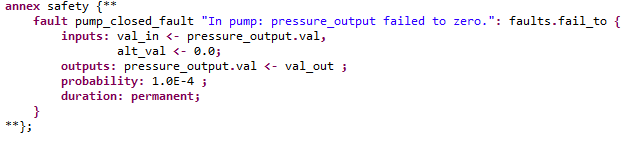
\includegraphics[trim=0 330 150 0,clip,width=1.0\textwidth]{images/pump_fault.png}
		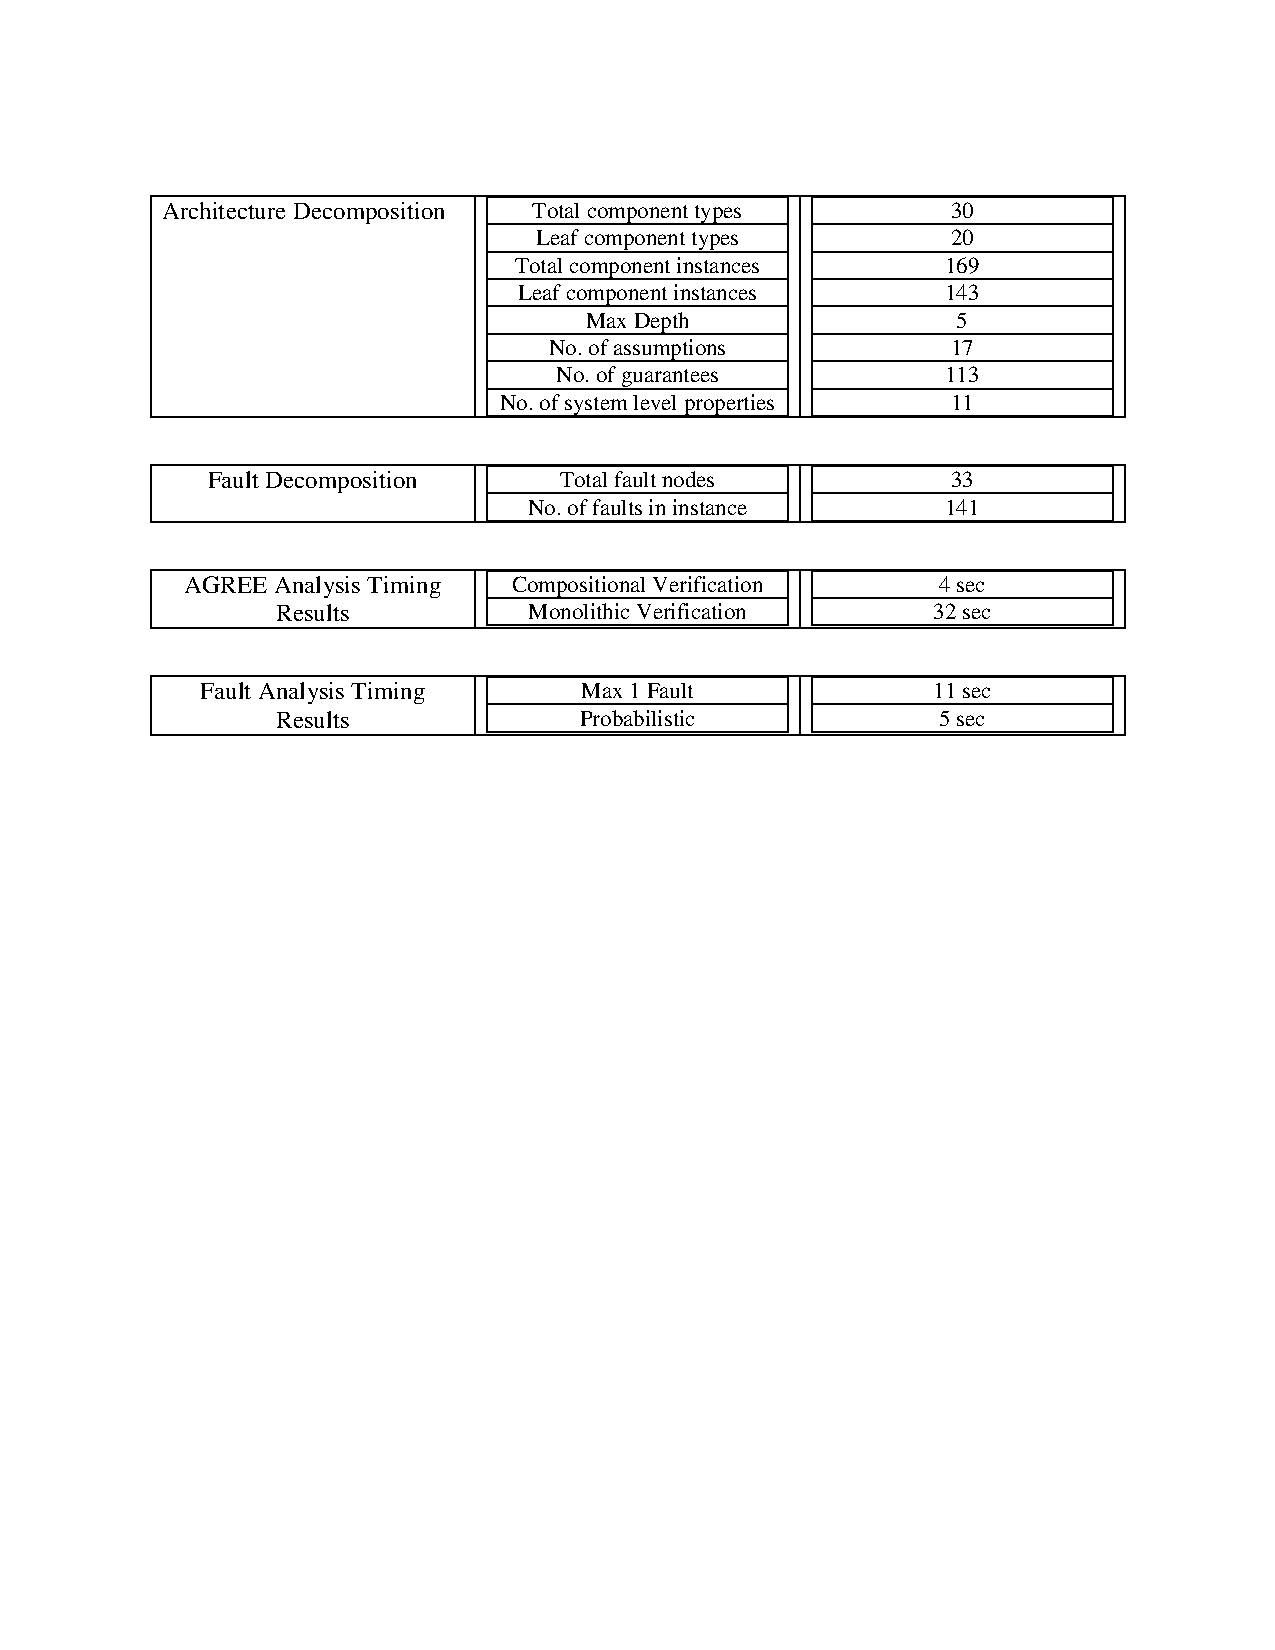
\includegraphics[trim=0 435 0 90,clip,width=1.0\textwidth]{images/arch_table.pdf}
		\caption{Modeling, Verification, and Fault Analysis Metrics}
 		\label{fig:metrics}
	\end{center}
	\vspace{-0.40in}
\end{figure}
\fi


Fault analysis on the top level WBS system was performed on 11 top-level properties using two fault hypotheses: the first allows at most one fault and the second allows combinations of faults that exceed the acceptable probabilities for the top-level hazard defined in ARP4761~\cite{SAE:ARP4761}.

We examine scalability by looking at analysis times for both compositional verification, where the verification task is split into layers to be analyzed separately, and monolithic verification, where the entire system is analyzed in one pass.  When considering the nominal system behavior (no faults), the total time required for analysis using compositional verification is 2 minutes 38 seconds, and the time for monolithic analysis is 30 seconds.  This nominal model is too small to gain significant benefit from compositional analysis.  However, when we consider faulty behavior, when given a single-fault hypothesis, the total time for compositional analysis is 2 minutes 37 seconds, and monolithic analysis did not finish after 42 minutes (ended due to out of memory error), clearly demonstrating the value of compositional analysis for more complex models.  Similarly, for probabilistic analysis, the compositional time is 2 minutes 38 seconds and the monolithic time is 3 minutes 31 seconds.

In our analysis, we discovered that most properties pass the model, but the \textit{Inadvertent braking at the wheel} properties were not resilient to a single fault nor did they meet the desired $10^{-9}$ fault threshold for probabilistic analysis.  In our model (as in the NuSMV model~\cite{DBLP:conf/cav/BozzanoCPJKPRT15}), there is a single pedal position sensor for the brake pedal.  If this sensor fails, it can command braking without a pilot request.  It was straightforward for us to diagnose the cause of the property failure using an automatically generated {\em counterexample}, which is a test case that demonstrates the failure.

This counterexample can be used to further iterate system design.  For our model, it could be that the time in the V1 phase of flight is short enough that we need to adjust our model failure rates for the V1 time scale, or that redundant sensors are required on the pedals (here we note that the architecture of the pedal assembly is not discussed in ARP4761).  It is straightforward and computationally inexpensive to run the analysis, allowing quick iterations between systems and safety engineers. As indicated in Figure~\ref{fig:interaction_with_FTA}, the sync and update between the preliminary system FTA and the architecture/analysis model continues until the system safety property is satisfied with the desired fault tolerance and failure probability achieved.

%In terms of the safety analysis process, this corresponds with an update in the preliminary system FTA which will eventually change the system FTA and impact SSA results.\mike{keep last sentence?}

%Mike: with regard to the safety process sentence at the end of the WBS case study, he thinks that we can keep that sentence, but update it to mention that we can iteratively run analysis if we don't achieve the desired fault tolerance for single failure or achieve the desired probability


\subsection{Quad-Redundant Flight Control System}
In order to discuss Byzantine faults and hardware failures with their propagations, we applied the Safety Annex to the Quad-Redundant Flight Control System (QFCS) model~\cite{QFCS15:backes}. Faulty behaviors were introduced in order to see the response of the system to several faults, and to evaluate fault mitigation logic in the model. The QFCS system-level properties failed when unhandled faulty behaviors were introduced.

We also used the Safety Annex to explore more complicated faults at the system level on a simplified QFCS model with cross-channel communication between its Flight Control Computers.

\begin{itemize}
	\item Byzantine faults~\cite{Driscoll-Byzantine-Fault} were simulated by creating one-to-one connections from the source to multiple observers so that disagreements could be introduced by injecting faults on individual outputs. The system level property ``at most one flight control computer in command'' was verified false in one second in the presence of Byzantine faults on the baseline model. The same property was verified in three seconds on an extended model with a Byzantine fault handling protocol.  System designers can use this approach to verify if a system design is resilient to Byzantine faults, examine vulnerabilities, and test if a mitigation mechanism works.

%original wording:	
	% A system-level property failed due to the fault on the baseline model, but did not fail on the model with Byzantine fault handling protocol added. Using the Safety Annex like this can test a system's vulnerability to Byzantine faults and verify mitigation mechanisms.
	
	\item Dependent faults were modeled by first injecting failures to the cross-channel data link (CCDL) bus (physical layer), and faults to the flight control computer (FCC) outputs (logical layer), then specifying fault propagations in the top level system implementation (where the data connections between FCC outputs were bound to the CCDL bus subcomponents). The fault propagation indicates that one CCDL bus failure can trigger all FCC output faults. With the fault hypothesis that maximum one fault active during execution, the system level property ``not all FCCs fail at the same time'' was verified false in one second.
	
%original wording:
%Dependent faults were modeled by injecting failures to hardware components (physical layer), and faults to software components (logical layer) that are bound to the hardware components, then specifying fault propagations at the QFCS system level to indicate that the software faults are dependent on the hardware failures. 	
\end{itemize}

%\mike{Results?} \janet{updated the last two paragraphs}
